% ============================================================
%  exercise_report.tex
%  Compile with: xelatex exercise_report.tex
% ============================================================
\documentclass[12pt, a4paper]{article}

% ── Typography & Language ──────────────────────────────────
\usepackage{fontspec}
\usepackage{polyglossia}
\setmainlanguage{vietnamese}
\setotherlanguage{english}
\setmainfont{Times New Roman}
\setsansfont{Arial}
\setmonofont{Courier New}

% ── Page Layout ────────────────────────────────────────────
\usepackage[top=2.5cm, bottom=2.5cm, left=3cm, right=2.5cm]{geometry}
\usepackage{setspace}
\onehalfspacing

% ── Math ───────────────────────────────────────────────────
\usepackage{amsmath, amssymb}

% ── Tables ─────────────────────────────────────────────────
\usepackage{booktabs}
\usepackage{tabularx}
\usepackage{array}
\usepackage{multirow}
\usepackage{longtable}

% ── Figures ────────────────────────────────────────────────
\usepackage{graphicx}
\graphicspath{{../results/plots/}}
\usepackage{float}
\usepackage{caption}
\usepackage{subcaption}

% ── Colors ─────────────────────────────────────────────────
\usepackage[dvipsnames, table]{xcolor}
\definecolor{codebg}{RGB}{248,248,248}
\definecolor{codeframe}{RGB}{200,200,200}
\definecolor{hcmutblue}{RGB}{0,70,127}
\definecolor{rowgray}{RGB}{240,240,240}

% ── Code Listings ──────────────────────────────────────────
\usepackage{listings}
\lstdefinestyle{pythonstyle}{
  language=Python,
  backgroundcolor=\color{codebg},
  frame=single,
  rulecolor=\color{codeframe},
  basicstyle=\footnotesize\ttfamily,
  keywordstyle=\color{blue}\bfseries,
  commentstyle=\color{OliveGreen}\itshape,
  stringstyle=\color{BrickRed},
  numbers=left,
  numberstyle=\tiny\color{gray},
  numbersep=8pt,
  tabsize=4,
  showstringspaces=false,
  breaklines=true,
  breakatwhitespace=true,
  captionpos=b,
  literate=
    {à}{{\`a}}1 {á}{{\'a}}1 {ả}{{\h{a}}}1 {ã}{{\~a}}1 {ạ}{{\d{a}}}1
    {ă}{{\u{a}}}1 {ắ}{{\'{\u{a}}}}1 {ằ}{{\`{\u{a}}}}1 {ẳ}{{\h{\u{a}}}}1
    {ẵ}{{\~{\u{a}}}}1 {ặ}{{\d{\u{a}}}}1
    {â}{{\^a}}1  {ấ}{{\'{\^a}}}1 {ầ}{{\`{\^a}}}1 {ẩ}{{\h{\^a}}}1
    {ẫ}{{\~{\^a}}}1 {ậ}{{\d{\^a}}}1
    {đ}{{\dj{}}}1
    {è}{{\`e}}1 {é}{{\'e}}1 {ẻ}{{\h{e}}}1 {ẽ}{{\~e}}1 {ẹ}{{\d{e}}}1
    {ê}{{\^e}}1  {ế}{{\'{\^e}}}1 {ề}{{\`{\^e}}}1 {ể}{{\h{\^e}}}1
    {ễ}{{\~{\^e}}}1 {ệ}{{\d{\^e}}}1
    {ì}{{\`i}}1 {í}{{\'i}}1 {ỉ}{{\h{i}}}1 {ĩ}{{\~i}}1 {ị}{{\d{i}}}1
    {ò}{{\`o}}1 {ó}{{\'o}}1 {ỏ}{{\h{o}}}1 {õ}{{\~o}}1 {ọ}{{\d{o}}}1
    {ô}{{\^o}}1  {ố}{{\'{\^o}}}1 {ồ}{{\`{\^o}}}1 {ổ}{{\h{\^o}}}1
    {ỗ}{{\~{\^o}}}1 {ộ}{{\d{\^o}}}1
    {ơ}{{\ohorn}}1 {ớ}{{\'{\ohorn}}}1 {ờ}{{\`{\ohorn}}}1
    {ở}{{\h{\ohorn}}}1 {ỡ}{{\~{\ohorn}}}1 {ợ}{{\d{\ohorn}}}1
    {ù}{{\`u}}1 {ú}{{\'u}}1 {ủ}{{\h{u}}}1 {ũ}{{\~u}}1 {ụ}{{\d{u}}}1
    {ư}{{\uhorn}}1 {ứ}{{\'{\uhorn}}}1 {ừ}{{\`{\uhorn}}}1
    {ử}{{\h{\uhorn}}}1 {ữ}{{\~{\uhorn}}}1 {ự}{{\d{\uhorn}}}1
    {ỳ}{{\`y}}1 {ý}{{\'y}}1 {ỷ}{{\h{y}}}1 {ỹ}{{\~y}}1 {ỵ}{{\d{y}}}1
    {Đ}{{\DJ{}}}1
    {→}{{$\rightarrow$}}1 {×}{{$\times$}}1 {│}{{|}}1 {▼}{{$\downarrow$}}1
    {──}{{\textemdash}}1
}
\lstset{style=pythonstyle}

\lstdefinestyle{plainstyle}{
  backgroundcolor=\color{codebg},
  frame=single,
  rulecolor=\color{codeframe},
  basicstyle=\footnotesize\ttfamily,
  numbers=none,
  breaklines=true,
  captionpos=b,
  literate=
    {→}{{$\rightarrow$}}1 {×}{{$\times$}}1 {│}{{|}}1 {▼}{{$\downarrow$}}1
    {──}{{\textemdash}}1
}

% ── Hyperlinks ─────────────────────────────────────────────
\usepackage[colorlinks=true, linkcolor=hcmutblue, urlcolor=hcmutblue, citecolor=hcmutblue]{hyperref}

% ── Misc ───────────────────────────────────────────────────
\usepackage{enumitem}
\usepackage{mdframed}
\usepackage{fancyhdr}
\usepackage{titlesec}
\usepackage{parskip}

% ── Section styling ────────────────────────────────────────
\titleformat{\section}{\large\bfseries\color{hcmutblue}}{}{0em}{\thesection.\quad}
\titleformat{\subsection}{\normalsize\bfseries}{}{0em}{\thesubsection\quad}
\titleformat{\subsubsection}{\normalsize\bfseries}{}{0em}{\thesubsubsection\quad}

% ── Header / Footer ────────────────────────────────────────
\pagestyle{fancy}
\fancyhf{}
\lhead{\small CO5085 – Học sâu và ứng dụng trong thị giác máy tính}
\rhead{\small Nguyễn Trung Phong}
\cfoot{\thepage}
\renewcommand{\headrulewidth}{0.4pt}

% ── Blockquote environment ─────────────────────────────────
\newmdenv[
  leftmargin=0pt,
  rightmargin=0pt,
  innerleftmargin=12pt,
  innerrightmargin=8pt,
  innertopmargin=6pt,
  innerbottommargin=6pt,
  linewidth=3pt,
  linecolor=hcmutblue,
  topline=false, bottomline=false, rightline=false,
  backgroundcolor=blue!4
]{myquote}

% ============================================================
\begin{document}

% ── Title Page ─────────────────────────────────────────────
\begin{titlepage}
  \centering
  \vspace*{1cm}
  {\large\bfseries ĐẠI HỌC BÁCH KHOA TP.HCM\\[0.3em]
   KHOA KHOA HỌC VÀ KỸ THUẬT MÁY TÍNH}\\[2em]
  \rule{\textwidth}{1.5pt}\\[0.5em]
  {\LARGE\bfseries\color{hcmutblue} BÁO CÁO BÀI TẬP}\\[0.5em]
  {\Large Phân loại Ảnh với các Mô hình Học Sâu Cơ bản}\\[0.5em]
  \rule{\textwidth}{1.5pt}\\[2.5em]

  \begin{tabular}{ll}
    \textbf{Môn học}    & CO5085 – Học sâu và ứng dụng trong thị giác máy tính \\[0.4em]
    \textbf{Sinh viên}  & Nguyễn Trung Phong – MSSV: 2570047 \\[0.4em]
    \textbf{Giảng viên} & Lê Thành Sách \\[0.4em]
    \textbf{Học kỳ}     & 2, năm học 2025–2026 \\[0.4em]
    \textbf{Deadline}   & 01/04/2026 \\[0.4em]
    \textbf{Repository} & \href{https://github.com/PhongNguyenTrung/hcmut-deeplearning-ass1/tree/main/exercise}{\texttt{GitHub/exercise}} \\
  \end{tabular}

  \vfill
  {\small Báo cáo hoàn thành ngày 31/03/2026}
\end{titlepage}

% ── Table of Contents ──────────────────────────────────────
\tableofcontents
\newpage

% ============================================================
\section{Giới thiệu}
% ============================================================

\subsection{Mục tiêu bài toán}

\textbf{Phân loại ảnh} (\textit{Image Classification}) là bài toán gán nhãn cho một ảnh đầu vào --- trả lời câu hỏi \textit{``ảnh này thuộc lớp nào?''}. Đây là bài toán nền tảng và quan trọng nhất của Thị giác Máy tính (\textit{Computer Vision}).

\begin{lstlisting}[style=plainstyle]
Dau vao: anh [H x W x C]  ->  Mo hinh  ->  Dau ra: nhan lop
\end{lstlisting}

Ứng dụng thực tế: nhận dạng khuôn mặt, chẩn đoán hình ảnh y tế, phân loại sản phẩm lỗi trong sản xuất, hệ thống xe tự lái nhận diện biển báo giao thông.

\textbf{Các mô hình được sử dụng trong bài tập này:}

\begin{table}[H]
\centering
\caption{Danh sách các mô hình được xây dựng}
\begin{tabular}{llc}
\toprule
\textbf{Mô hình} & \textbf{Kiến trúc} & \textbf{Phần} \\
\midrule
Softmax Regression          & Tuyến tính thuần tuý      & 1 \\
MLP (Multi-Layer Perceptron)& Fully-connected           & 1 \\
CNN (Convolutional Neural Network) & Tích chập cục bộ  & 1 \\
Vision Transformer (ViT) --- PyTorch & Self-Attention   & 1 \\
CustomViT (tự xây từ \texttt{einsum}) & Self-Attention  & 3 \\
CNN + Transformer Hybrid    & Hybrid                    & 4 \\
SpatialToken ViT            & Attention trên pixel      & 4 \\
ChannelToken ViT            & Attention trên channel    & 4 \\
LSTM / GRU                  & Recurrent                 & 5 \\
\bottomrule
\end{tabular}
\end{table}

Tất cả mô hình được huấn luyện \textbf{from scratch} (không pretrained weights) trên \textbf{CIFAR-100} với training loop tự viết bằng PyTorch.

\subsection{Mục tiêu học tập}

Bài tập này nhắm đến ba mục tiêu học tập chính:

\begin{enumerate}
  \item \textbf{So sánh các kiến trúc từ đơn giản đến phức tạp:} Từ Softmax Regression tuyến tính $\rightarrow$ MLP $\rightarrow$ CNN $\rightarrow$ ViT $\rightarrow$ Hybrid, để thấy rõ sự tiến bộ và trade-off giữa các phương pháp qua từng giai đoạn lịch sử học sâu.

  \item \textbf{Hiểu training loop:} Tự viết vòng lặp huấn luyện PyTorch --- \texttt{zero\_grad $\rightarrow$ forward $\rightarrow$ loss $\rightarrow$ backward $\rightarrow$ clip $\rightarrow$ step} --- thay vì dùng API cấp cao, để hiểu cơ chế tối ưu hoá từ gốc.

  \item \textbf{Hiểu cơ chế Transformer:} Tự hiện thực \texttt{MultiHeadAttention} và \texttt{TransformerEncoderLayer} từ \texttt{nn.Linear}, \texttt{LayerNorm}, \texttt{torch.einsum} --- không dùng module có sẵn --- để nắm vững toán học bên trong attention.
\end{enumerate}

% ============================================================
\section{Dataset}
% ============================================================

\subsection{Dataset sử dụng}

Bài tập này sử dụng \textbf{CIFAR-100} (Canadian Institute For Advanced Research, 100 classes).

\begin{table}[H]
\centering
\caption{Thông tin tập dữ liệu CIFAR-100}
\begin{tabular}{ll}
\toprule
\textbf{Thuộc tính} & \textbf{Giá trị} \\
\midrule
Tên               & CIFAR-100 \\
Số lớp (fine-grained) & 100 \\
Số superclass     & 20 \\
Kích thước ảnh    & $32 \times 32$ pixels, 3 kênh RGB \\
Tổng số ảnh       & 60,000 \\
Train / Validation / Test & 45,000 / 5,000 / 10,000 \\
Ảnh mỗi lớp (train) & 450 \\
\bottomrule
\end{tabular}
\end{table}

\subsection{Lý do chọn}

CIFAR-100 được chọn thay vì CIFAR-10 (mặc định trong đề bài) để bài toán đủ khó nhằm phân biệt rõ ràng năng lực từng kiến trúc:

\begin{table}[H]
\centering
\caption{So sánh CIFAR-10 và CIFAR-100}
\begin{tabular}{lll}
\toprule
\textbf{Tiêu chí} & \textbf{CIFAR-10} & \textbf{CIFAR-100 (được chọn)} \\
\midrule
Số lớp                       & 10          & 100 \\
Ảnh mỗi lớp (train)          & 5,000       & 500 \\
Độ khó                       & Thấp        & Trung bình--cao \\
Softmax Regression đạt       & $\sim$70--75\% & $\sim$8\% \\
Phân biệt kiến trúc?         & Khó (tất cả đều cao) & Rõ ràng \\
\bottomrule
\end{tabular}
\end{table}

Với CIFAR-10, ngay cả Softmax Regression đạt $\sim$70\% nên không thể thấy sự khác biệt giữa các kiến trúc. CIFAR-100 với 100 lớp fine-grained (ví dụ: baby, boy, girl, man, woman --- 5 lớp riêng biệt trong superclass ``people'') làm bài toán đủ thử thách.

\subsection{Preprocessing}

\begin{lstlisting}[language=Python, caption={Data transforms cho CIFAR-100}]
# Chuan hoa voi thong ke CIFAR-100 (KHONG dung ImageNet stats)
mean = [0.5071, 0.4867, 0.4408]
std  = [0.2675, 0.2565, 0.2761]

# Tap train -- co augmentation
train_transforms = transforms.Compose([
    transforms.RandomCrop(32, padding=4),
    transforms.RandomHorizontalFlip(),
    transforms.ToTensor(),
    transforms.Normalize(mean, std),
])

# Tap validation / test -- chi chuan hoa
eval_transforms = transforms.Compose([
    transforms.ToTensor(),
    transforms.Normalize(mean, std),
])
\end{lstlisting}

\begin{myquote}
\textbf{Tại sao dùng CIFAR-100 stats thay vì ImageNet stats?} CIFAR-100 (ảnh $32\times32$ vật thể) và ImageNet (ảnh tự nhiên lớn) có phân phối màu khác nhau. Dùng sai stats làm dữ liệu bị chuẩn hoá sai, ảnh hưởng đến tốc độ hội tụ và kết quả.
\end{myquote}

% ============================================================
\section{Phương pháp}
% ============================================================

\textbf{Quy ước chung:} Mọi mô hình nhận input \texttt{[B, 3, 32, 32]} và trả về logits \texttt{[B, 100]}. Không thêm softmax trong \texttt{forward()} vì \texttt{nn.CrossEntropyLoss} đã tích hợp \texttt{log\_softmax} bên trong.

% ── 3.1 ──────────────────────────────────────────────────
\subsection{Phần 1 --- Các mô hình cơ bản}

\subsubsection{Softmax Regression}

\textbf{Ý tưởng:} Mô hình tuyến tính đơn giản nhất. Ánh xạ trực tiếp từ raw pixels đến xác suất lớp qua một lớp tuyến tính duy nhất.

\textbf{Kiến trúc:}
\begin{lstlisting}[style=plainstyle]
Dau vao: [B, 3, 32, 32]
    |
    v
Flatten -> [B, 3072]    (3x32x32 = 3072 features)
    |
    v
Linear(3072 -> 100) -> [B, 100]   logits
\end{lstlisting}

\textbf{Code:}
\begin{lstlisting}[language=Python]
self.net = nn.Sequential(
    nn.Flatten(),
    nn.Linear(3*32*32, num_classes),
)
\end{lstlisting}

\begin{table}[H]
\centering
\caption{Thông số Softmax Regression}
\begin{tabular}{ll}
\toprule
\textbf{Tham số} & \textbf{Giá trị} \\
\midrule
Input dim      & $3 \times 32 \times 32 = 3{,}072$ \\
Số tham số     & $3{,}072 \times 100 + 100 = \mathbf{307{,}300}$ \\
Activation     & Không (softmax tích hợp trong Loss) \\
Hạn chế        & Chỉ học biên quyết định tuyến tính \\
\bottomrule
\end{tabular}
\end{table}

\subsubsection{MLP (Multi-Layer Perceptron)}

\textbf{Ý tưởng:} Thêm các lớp ẩn với hàm kích hoạt phi tuyến ReLU để học được các pattern phức tạp hơn. BatchNorm và Dropout giúp ổn định training và giảm overfitting.

\textbf{Kiến trúc:}
\begin{lstlisting}[style=plainstyle]
Dau vao: [B, 3, 32, 32]
    |
    v Flatten -> [B, 3072]
    |
    v Linear(3072->512) -> BN -> ReLU -> Dropout(0.3)
    |
    v Linear(512->256)  -> BN -> ReLU -> Dropout(0.3)
    |
    v Linear(256->100) -> [B, 100]
\end{lstlisting}

\begin{table}[H]
\centering
\caption{Thông số MLP}
\begin{tabular}{ll}
\toprule
\textbf{Tham số} & \textbf{Giá trị} \\
\midrule
Lớp ẩn         & 2 (512 $\rightarrow$ 256 neurons) \\
Activation     & ReLU \\
Regularization & BatchNorm1d + Dropout(0.3) \\
Số tham số     & $\sim$\textbf{1.7M} \\
\bottomrule
\end{tabular}
\end{table}

\textbf{Hạn chế:} \texttt{Flatten} phá vỡ cấu trúc không gian 2D của ảnh. Pixel $(i, j)$ và pixel $(i, j+1)$ --- hai pixel kề nhau --- sau khi Flatten trở thành hai features độc lập, mạng không biết chúng ở cạnh nhau. CNN giải quyết vấn đề này.

\subsubsection{SimpleCNN (VGG-style)}

\textbf{Ý tưởng:} Khai thác cấu trúc không gian 2D của ảnh thông qua tích chập cục bộ. Mỗi filter chỉ ``nhìn'' vùng $3\times3$, học đặc trưng từ vùng lân cận rồi truyền lên lớp cao hơn.

\textbf{Kiến trúc:}
\begin{lstlisting}[style=plainstyle]
Dau vao: [B, 3, 32, 32]
    |
    v ConvBlock1: [Conv2d(3->32,3x3)+BN+ReLU]x2 -> MaxPool(2) [B,32,16,16]
    v ConvBlock2: [Conv2d(32->64,3x3)+BN+ReLU]x2 -> MaxPool(2) [B,64,8,8]
    v ConvBlock3: [Conv2d(64->128,3x3)+BN+ReLU]x2 -> MaxPool(2) [B,128,4,4]
    v AdaptiveAvgPool2d(1) -> Flatten -> [B, 128]
    |
    v Linear(128->256) -> ReLU -> Dropout(0.3) -> Linear(256->100)
[B, 100]
\end{lstlisting}

\begin{table}[H]
\centering
\caption{Thông số SimpleCNN}
\begin{tabular}{ll}
\toprule
\textbf{Tham số} & \textbf{Giá trị} \\
\midrule
Conv blocks    & 3 (channels: $3 \rightarrow 32 \rightarrow 64 \rightarrow 128$) \\
Kernel size    & $3\times3$, padding=1 \\
Pooling        & MaxPool(2) --- giảm spatial $1/2$ mỗi block \\
AdaptiveAvgPool & Pool $128\times4\times4 \rightarrow 128\times1\times1$ \\
Số tham số     & $\sim$\textbf{346.6K} \\
\bottomrule
\end{tabular}
\end{table}

\textbf{Ba lý do CNN vượt trội MLP với dữ liệu ảnh:}
\begin{enumerate}
  \item \textbf{Locality:} Mỗi filter chỉ xử lý vùng $3\times3$ --- học đặc trưng cục bộ như cạnh, góc, texture.
  \item \textbf{Weight sharing:} Cùng bộ filter áp dụng tại mọi vị trí $\rightarrow$ giảm params, tổng quát hoá tốt hơn.
  \item \textbf{Hierarchical features:} Block 1 học edges, Block 2 học shapes, Block 3 học objects.
\end{enumerate}

\subsubsection{Vision Transformer (dùng PyTorch built-in)}

\textbf{Ý tưởng:} Chia ảnh thành các ``patches'' nhỏ rồi xử lý như chuỗi tokens qua Transformer --- tương tự cách xử lý câu trong NLP.

\textbf{Kiến trúc:}
\begin{lstlisting}[style=plainstyle]
Dau vao: [B, 3, 32, 32]
    |
    v Patch Embedding (Conv2d kernel=4, stride=4)
[B, 128, 8, 8] -> flatten+transpose -> [B, 64, 128]
    64 patches, moi patch 4x4 pixels, embed thanh 128-dim vector
    |
    v Prepend CLS token -> [B, 65, 128]
    v + Positional Encoding [1, 65, 128] (learnable)
    v TransformerEncoder: 4 layers, d_model=128, nhead=4, ffn=512, Pre-LN
    v CLS token -> LayerNorm -> Linear(128->100)
[B, 100]
\end{lstlisting}

\begin{table}[H]
\centering
\caption{Thông số SimpleViT}
\begin{tabular}{ll}
\toprule
\textbf{Tham số} & \textbf{Giá trị} \\
\midrule
Patch size          & $4\times4$ ($\rightarrow$ 64 patches trên ảnh $32\times32$) \\
$d_\text{model}$    & 128 \\
Số attention heads  & 4 (mỗi head: 32-dim) \\
Số Transformer layers & 4 \\
FFN dimension       & 512 ($= 4 \times d_\text{model}$) \\
Positional Encoding & Learnable \\
LayerNorm           & Pre-LN \\
Số tham số          & $\sim$\textbf{821.0K} \\
\bottomrule
\end{tabular}
\end{table}

\begin{myquote}
\textbf{Tại sao patch\_size=4 không phải 16?} ViT-B/16 gốc dùng patch $16\times16$ cho ảnh $224\times224$ $\rightarrow$ 196 patches. Với ảnh $32\times32$: patch $16\times16$ $\rightarrow$ chỉ \textbf{4 patches} (quá ít). Patch $4\times4$ $\rightarrow$ \textbf{64 patches} --- cân bằng giữa số lượng và độ phong phú mỗi patch.
\end{myquote}

% ── 3.2 ──────────────────────────────────────────────────
\subsection{Phần 2 --- Training \& Evaluation}

\subsubsection{Training loop}

Theo yêu cầu bài tập, \textbf{không dùng} Lightning \texttt{trainer.fit()} hay Keras-style API. Tự viết từng bước:

\begin{lstlisting}[language=Python, caption={Training loop một epoch}]
def train_one_epoch(model, loader, optimizer, criterion, device,
                    clip_norm=1.0):
    model.train()
    total_loss, total_correct, total_samples = 0, 0, 0

    for x, y in loader:
        x, y = x.to(device), y.to(device)

        # Buoc 1: Xoa gradient tu batch truoc
        optimizer.zero_grad()

        # Buoc 2: Forward pass
        logits = model(x)                    # [B, 100]

        # Buoc 3: Tinh loss
        loss = criterion(logits, y)

        # Buoc 4: Backpropagation
        loss.backward()

        # Buoc 5: Gradient clipping
        nn.utils.clip_grad_norm_(model.parameters(), clip_norm)

        # Buoc 6: Cap nhat tham so
        optimizer.step()

        total_loss    += loss.item() * x.size(0)
        total_correct += (logits.argmax(1) == y).sum().item()
        total_samples += x.size(0)

    return total_loss / total_samples, total_correct / total_samples
\end{lstlisting}

\textbf{Giải thích Gradient Clipping:} Nếu norm vector gradient vượt quá \texttt{max\_norm=1.0}, scale toàn bộ gradient xuống sao cho norm = 1.0. Kỹ thuật này ngăn ``exploding gradients'' --- đặc biệt quan trọng với RNN và Transformer.

\begin{lstlisting}[language=Python, caption={Vòng lặp huấn luyện fit()}]
def fit(model, train_loader, val_loader, config):
    optimizer = AdamW(model.parameters(), lr=config["lr"],
                      weight_decay=1e-4)
    scheduler = CosineAnnealingLR(optimizer,
                                   T_max=config["epochs"],
                                   eta_min=config["lr"]*0.01)
    best_val_acc, history = 0.0, defaultdict(list)
    for epoch in range(config["epochs"]):
        train_loss, train_acc = train_one_epoch(model, train_loader, ...)
        val_loss,   val_acc   = evaluate(model, val_loader, ...)
        scheduler.step()
        if val_acc > best_val_acc:
            best_val_acc = val_acc
            torch.save(model.state_dict(), config["save_path"])
    return history
\end{lstlisting}

\subsubsection{Metrics}

\begin{itemize}
  \item \textbf{Accuracy:} \% ảnh phân loại đúng trên tập test.
  \item \textbf{F1-macro:} Trung bình F1 của 100 lớp --- đánh giá đều trên tất cả lớp, không bị lớp lớn lấn át.
  \item \textbf{Loss:} CrossEntropyLoss --- đo độ tin cậy của xác suất dự đoán.
\end{itemize}

\subsubsection{Cấu hình Hyperparameters}

\begin{table}[H]
\centering
\caption{Hyperparameters Phần 1+2}
\begin{tabular}{llcccl}
\toprule
\textbf{Mô hình} & \textbf{LR} & \textbf{Batch} & \textbf{Epochs} & \textbf{Optimizer} & \textbf{Scheduler} \\
\midrule
SoftmaxRegression & 0.1   & 256 & 30  & AdamW & CosineAnnealing \\
MLP               & 1e-3  & 128 & 50  & AdamW & CosineAnnealing \\
SimpleCNN         & 1e-3  & 128 & 50  & AdamW & CosineAnnealing \\
SimpleViT         & 3e-4  & 128 & 100 & AdamW & CosineAnnealing \\
\bottomrule
\end{tabular}
\end{table}

\subsubsection{Kết quả so sánh}

\begin{figure}[H]
  \centering
  \begin{subfigure}[b]{0.48\textwidth}
    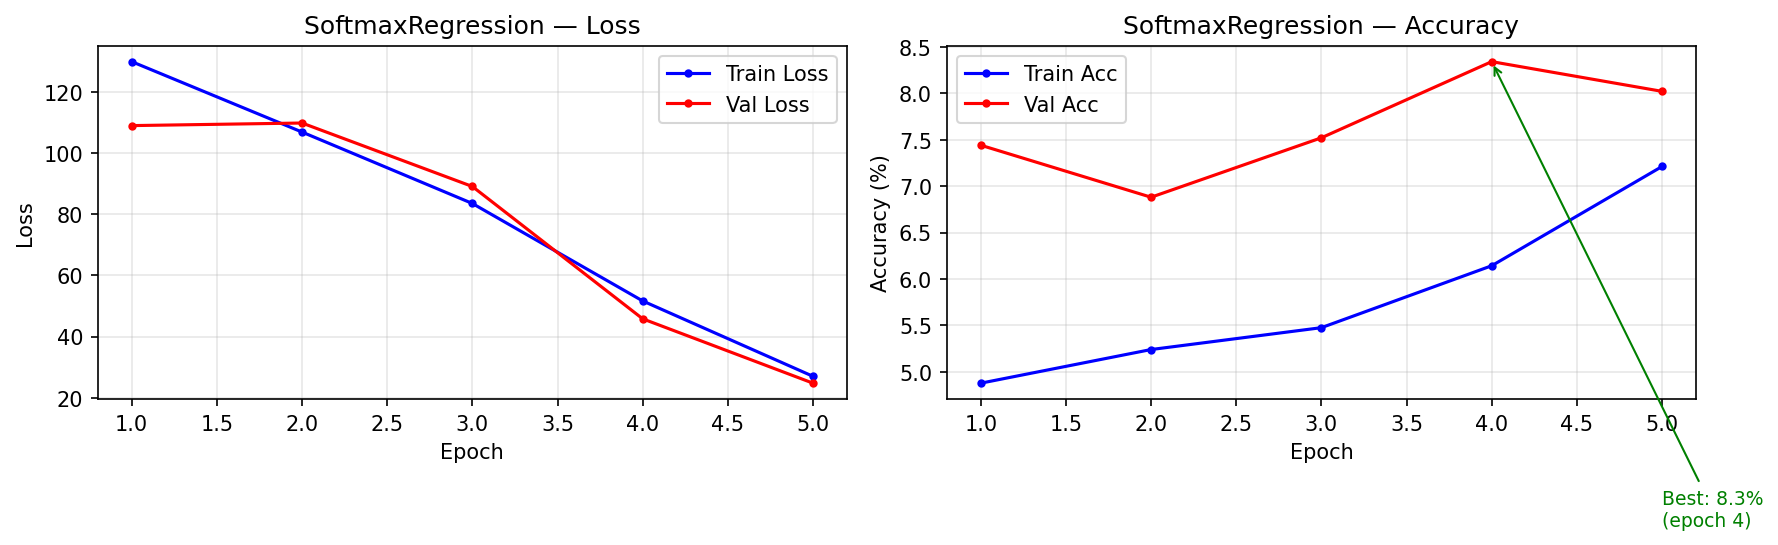
\includegraphics[width=\textwidth]{softmax_curves.png}
    \caption{Softmax Regression}
  \end{subfigure}
  \hfill
  \begin{subfigure}[b]{0.48\textwidth}
    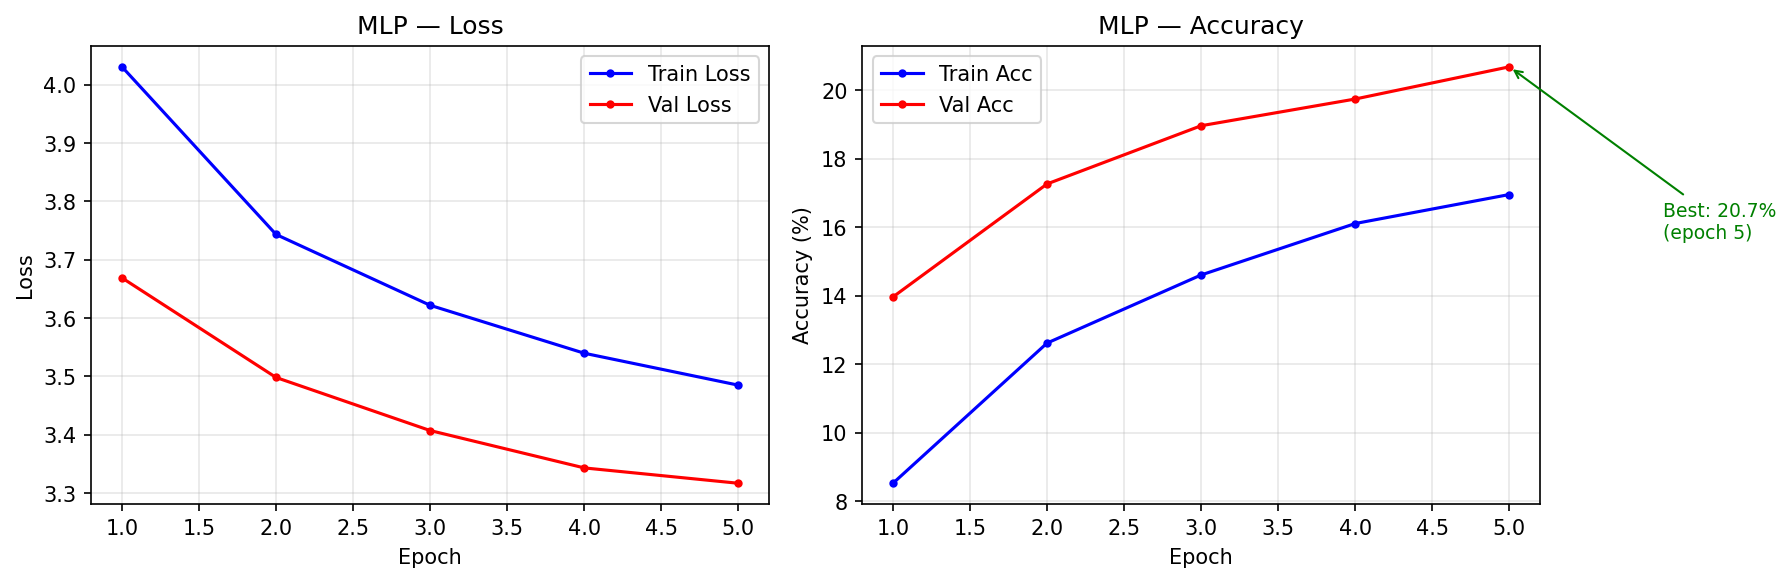
\includegraphics[width=\textwidth]{mlp_curves.png}
    \caption{MLP}
  \end{subfigure}

  \vspace{0.5em}
  \begin{subfigure}[b]{0.48\textwidth}
    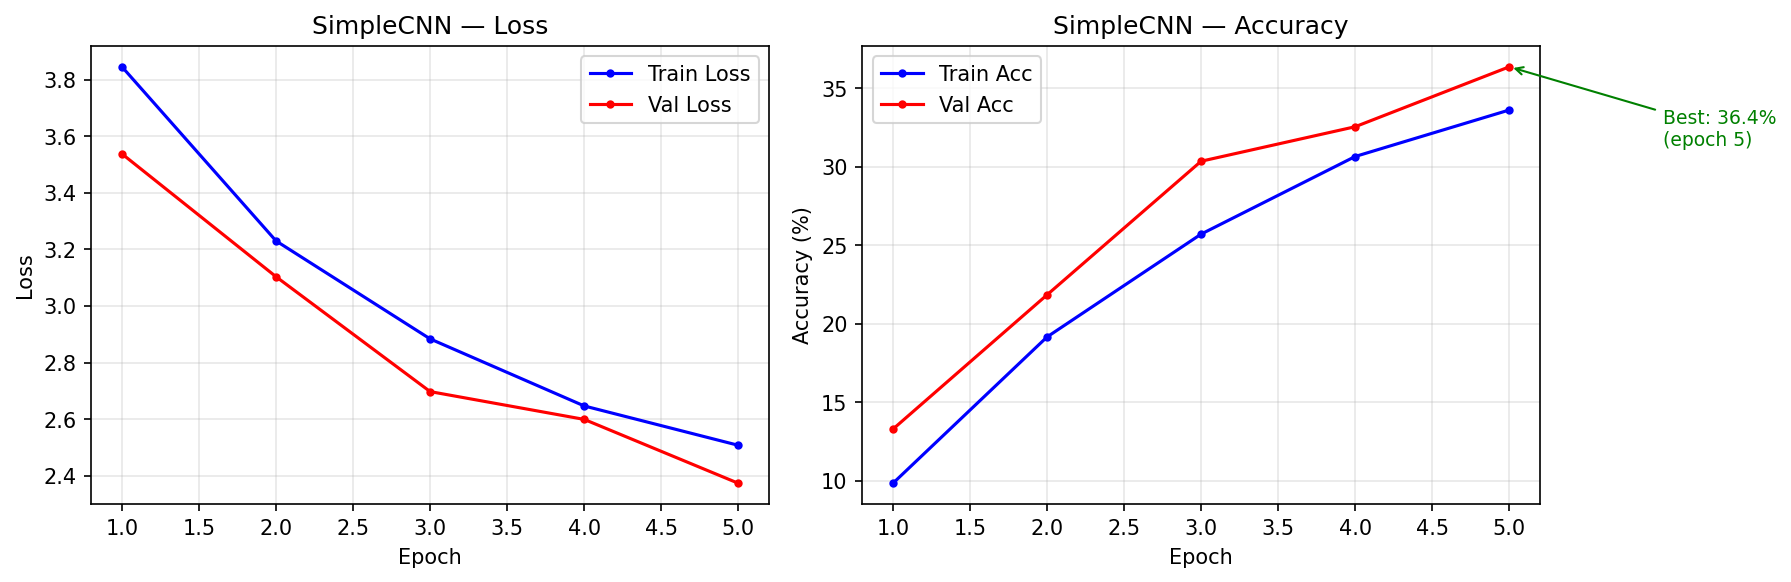
\includegraphics[width=\textwidth]{cnn_curves.png}
    \caption{SimpleCNN}
  \end{subfigure}
  \hfill
  \begin{subfigure}[b]{0.48\textwidth}
    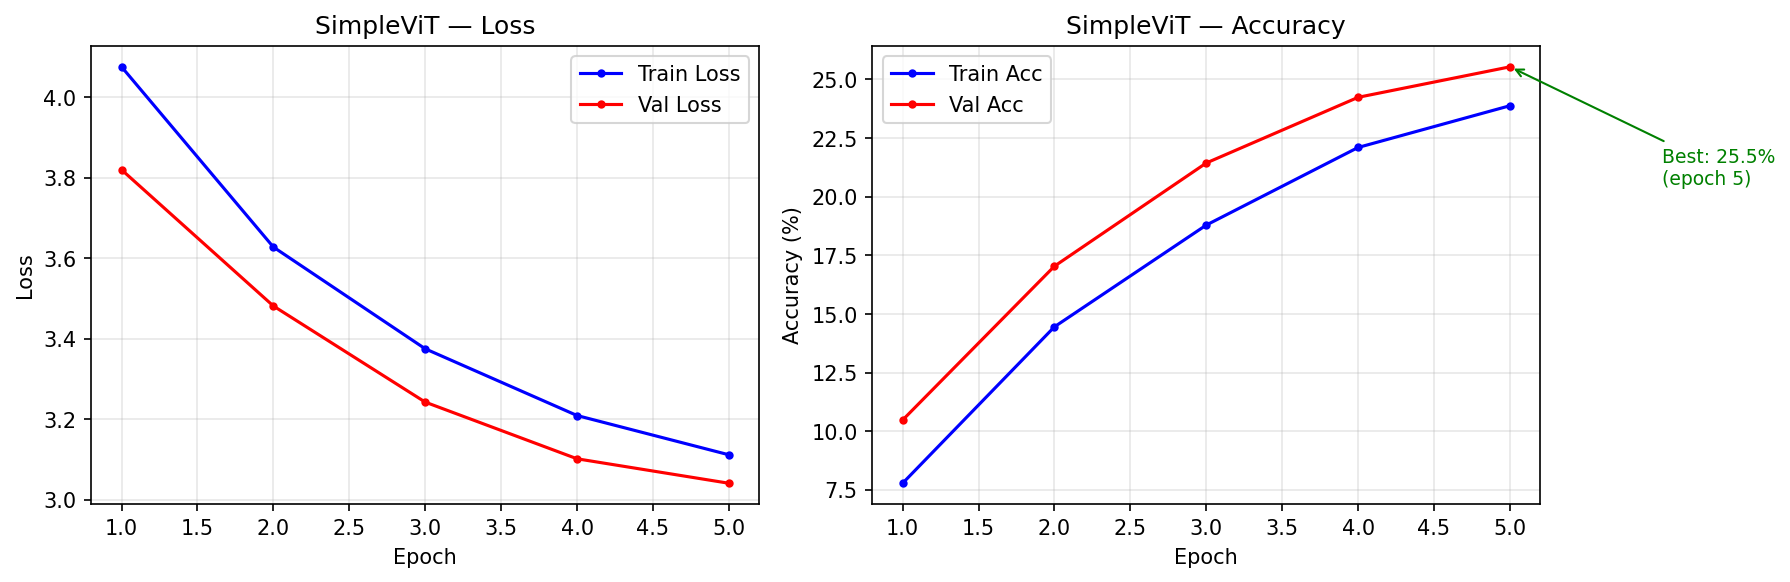
\includegraphics[width=\textwidth]{vit_curves.png}
    \caption{SimpleViT}
  \end{subfigure}
  \caption{Training curves của 4 mô hình Phần 1}
\end{figure}

\begin{figure}[H]
  \centering
  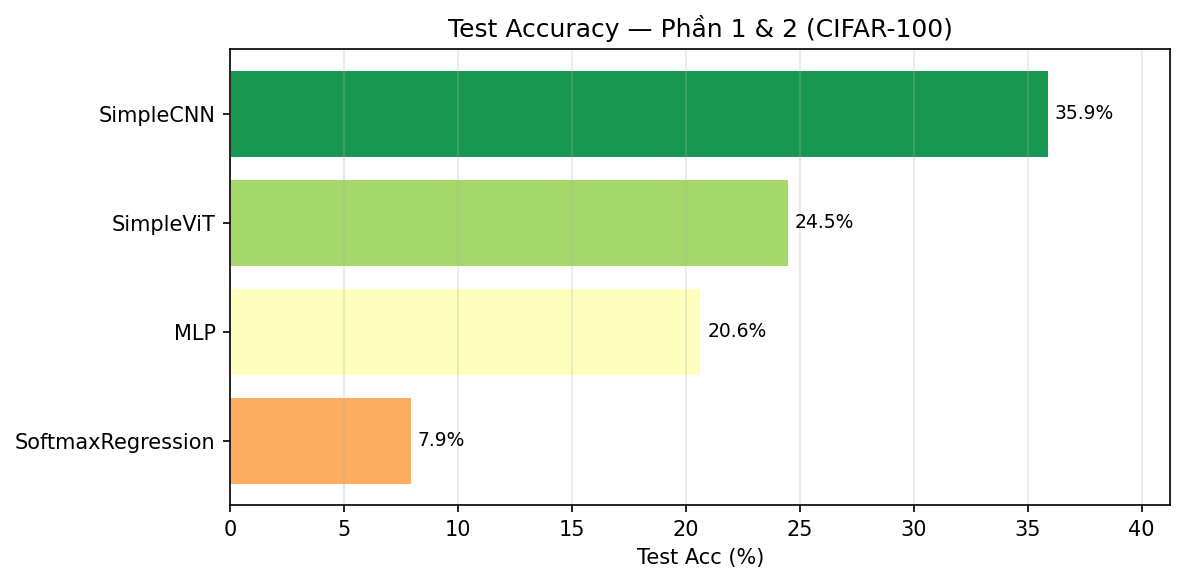
\includegraphics[width=0.75\textwidth]{part1_2_bar.png}
  \caption{So sánh Test Accuracy 4 mô hình Phần 1+2. SimpleCNN dẫn đầu với 35.88\%, gấp hơn $4\times$ Softmax Regression.}
\end{figure}

\begin{table}[H]
\centering
\caption{Kết quả 4 mô hình Phần 1+2 trên CIFAR-100 test set}
\rowcolors{2}{rowgray}{white}
\begin{tabular}{lccccc}
\toprule
\textbf{Mô hình} & \textbf{Test Acc} & \textbf{Val Acc} & \textbf{F1-macro} & \textbf{Params} & \textbf{Acc/Param} \\
\midrule
SoftmaxRegression & 7.94\%  & 8.34\%  & 6.09\%  & 307.3K  & 25.8\%/M \\
MLP               & 20.63\% & 20.68\% & 18.31\% & 1.7M    & 12.1\%/M \\
SimpleViT         & 24.47\% & 25.54\% & 22.35\% & 821.0K  & 29.8\%/M \\
\textbf{SimpleCNN}& \textbf{35.88\%} & \textbf{36.38\%} & \textbf{34.48\%} & \textbf{346.6K} & \textbf{103.5\%/M} \\
\bottomrule
\end{tabular}
\end{table}

\subsubsection{Nhận xét}

\textbf{Softmax Regression (7.94\%):} Chỉ học được biên quyết định tuyến tính trong không gian 3072-chiều --- chỉ tốt hơn random (1\%) khoảng 8 lần. F1-macro (6.09\%) thấp hơn accuracy (7.94\%) cho thấy mô hình tập trung vào vài lớp dễ, bỏ qua phần lớn lớp còn lại.

\textbf{MLP (20.63\%):} Các lớp ẩn với ReLU học được đặc trưng phi tuyến, cải thiện $2.6\times$ so với Softmax. Tuy nhiên \texttt{Flatten} phá vỡ quan hệ không gian 2D: hai pixels kề nhau bị xử lý như hai features độc lập.

\textbf{SimpleCNN (35.88\%) --- tốt nhất Phần 1:} CNN (346.6K params) vượt MLP (1.7M params) --- bằng chứng \textbf{inductive bias phù hợp quan trọng hơn số tham số}. Acc/Param = 103.5\%/M --- hiệu quả tốt nhất trong 4 mô hình.

\textbf{SimpleViT (24.47\%):} Thấp hơn CNN vì thiếu spatial inductive bias. Với 45K mẫu (450/lớp), Transformer chưa đủ data để vượt CNN. Val accuracy vẫn tăng ở epoch 100 $\rightarrow$ cần nhiều epochs hơn.

% ── 3.3 ──────────────────────────────────────────────────
\subsection{Phần 3 --- Transformer tự xây}

\subsubsection{Transformer Encoder (custom)}

Hiện thực TransformerEncoder \textbf{chỉ từ}: \texttt{nn.Linear}, \texttt{nn.LayerNorm}, \texttt{torch.einsum}, \texttt{F.softmax}, \texttt{F.dropout}. \textbf{Không được dùng}: \texttt{nn.MultiheadAttention}, \texttt{nn.TransformerEncoderLayer}.

\textbf{Lý thuyết Scaled Dot-Product Attention:}

\begin{align}
  Q &= X W_Q, \quad K = X W_K, \quad V = X W_V \\
  \text{Attention}(Q, K, V) &= \text{softmax}\!\left(\frac{QK^\top}{\sqrt{d_\text{head}}}\right) V
\end{align}

Chia $d_\text{model}=128$ thành $H=4$ heads, mỗi head có $d_\text{head}=32$.

\textbf{Multi-Head Attention bằng \texttt{torch.einsum}:}

\begin{lstlisting}[language=Python, caption={Custom Multi-Head Attention}]
class CustomMultiHeadAttention(nn.Module):
    def __init__(self, d_model, num_heads, dropout=0.1):
        self.W_q = nn.Linear(d_model, d_model, bias=False)
        self.W_k = nn.Linear(d_model, d_model, bias=False)
        self.W_v = nn.Linear(d_model, d_model, bias=False)
        self.W_o = nn.Linear(d_model, d_model)
        self.d_head = d_model // num_heads

    def forward(self, x):    # x: [B, T, d_model]
        B, T, _ = x.shape
        H, d_h = self.num_heads, self.d_head

        Q = self.W_q(x).reshape(B,T,H,d_h).transpose(1,2)
        K = self.W_k(x).reshape(B,T,H,d_h).transpose(1,2)
        V = self.W_v(x).reshape(B,T,H,d_h).transpose(1,2)

        # 'bhid,bhjd->bhij': batch, head, query_pos, key_pos, d_head
        scores = torch.einsum('bhid,bhjd->bhij', Q, K) / math.sqrt(d_h)
        attn   = F.softmax(scores, dim=-1)

        out = torch.einsum('bhij,bhjd->bhid', attn, V)
        out = out.transpose(1,2).reshape(B, T, self.d_model)
        return self.W_o(out)
\end{lstlisting}

\subsubsection{Pre-LN TransformerEncoderLayer}

\begin{lstlisting}[language=Python, caption={Custom TransformerEncoderLayer (Pre-LN)}]
class CustomTransformerEncoderLayer(nn.Module):
    def __init__(self, d_model, num_heads, ffn_dim=None, dropout=0.1):
        self.norm1 = nn.LayerNorm(d_model)
        self.norm2 = nn.LayerNorm(d_model)
        self.attn  = CustomMultiHeadAttention(d_model, num_heads, dropout)
        self.ffn   = nn.Sequential(
            nn.Linear(d_model, ffn_dim),
            nn.GELU(),
            nn.Dropout(dropout),
            nn.Linear(ffn_dim, d_model),
        )

    def forward(self, x):
        x = x + self.attn(self.norm1(x))   # Pre-LN residual
        x = x + self.ffn(self.norm2(x))
        return x
\end{lstlisting}

\begin{table}[H]
\centering
\caption{Pre-LN vs Post-LN}
\begin{tabular}{llll}
\toprule
\textbf{Variant} & \textbf{Công thức} & \textbf{Gradient} & \textbf{Warmup} \\
\midrule
Post-LN (Vaswani 2017) & $x = \text{LN}(x + \text{Attn}(x))$ & Không ổn định & Có \\
\textbf{Pre-LN (được chọn)} & $x = x + \text{Attn}(\text{LN}(x))$ & Ổn định từ đầu & Không \\
\bottomrule
\end{tabular}
\end{table}

\subsubsection{ViT tự xây}

Giống hệt SimpleViT (Phần 1) --- cùng patch embedding, CLS token, positional encoding, classification head --- \textbf{chỉ thay} \texttt{nn.TransformerEncoder} bằng \texttt{CustomTransformerEncoder}.

\subsubsection{So sánh}

\begin{figure}[H]
  \centering
  \begin{subfigure}[b]{0.55\textwidth}
    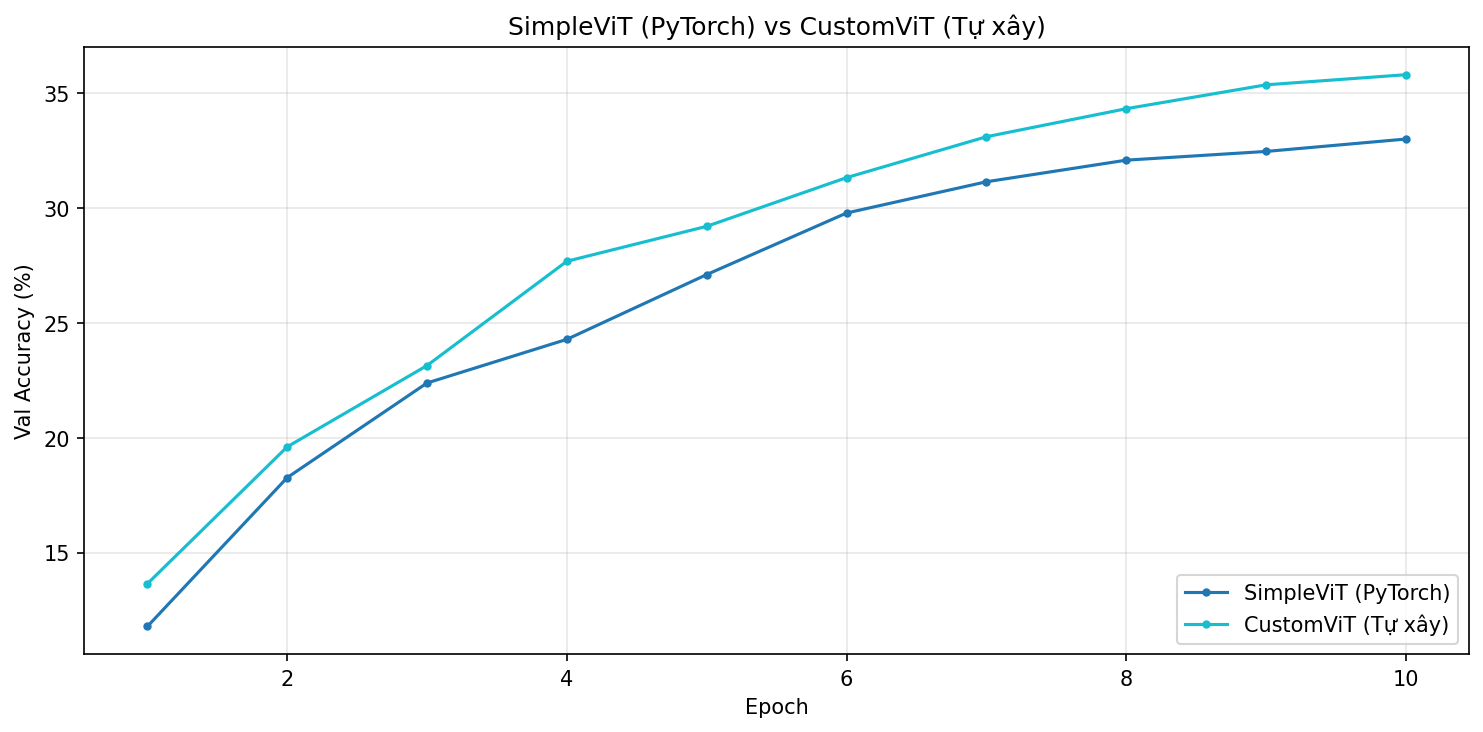
\includegraphics[width=\textwidth]{part3_comparison_curves.png}
    \caption{Training curves}
  \end{subfigure}
  \hfill
  \begin{subfigure}[b]{0.42\textwidth}
    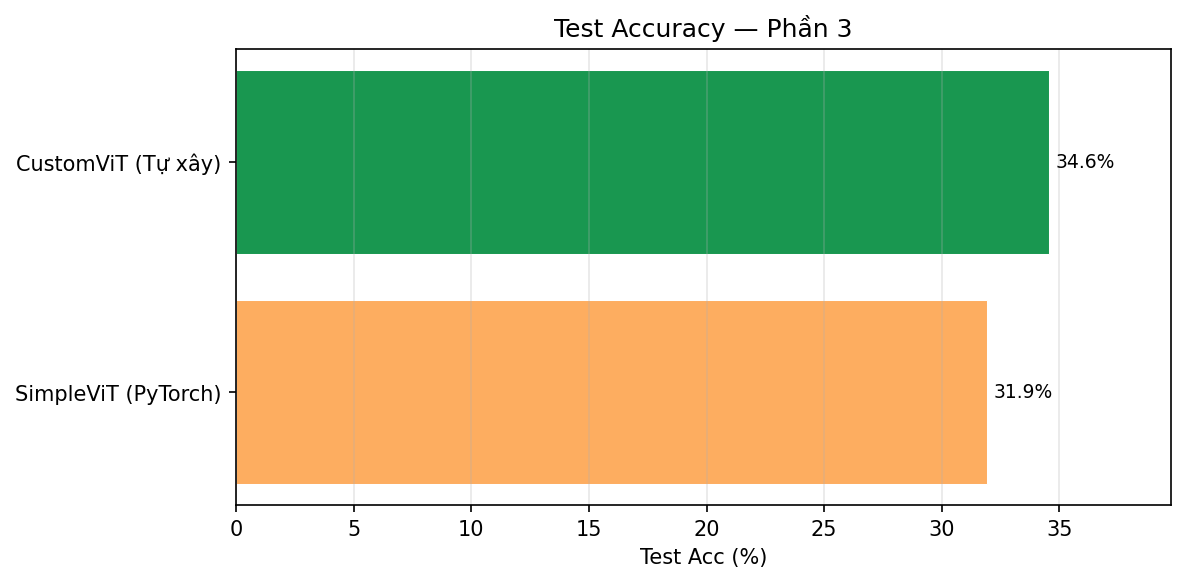
\includegraphics[width=\textwidth]{part3_bar.png}
    \caption{Test Accuracy}
  \end{subfigure}
  \caption{So sánh SimpleViT (PyTorch) và CustomViT (tự xây)}
\end{figure}

\begin{table}[H]
\centering
\caption{Kết quả Phần 3}
\rowcolors{2}{rowgray}{white}
\begin{tabular}{lllccccc}
\toprule
\textbf{Mô hình} & \textbf{Encoder} & \textbf{Test Acc} & \textbf{Val Acc} & \textbf{F1} & \textbf{Params} & \textbf{Time/ep} \\
\midrule
SimpleViT (PyTorch) & \texttt{nn.TransformerEncoder} & 31.92\% & 33.00\% & 30.39\% & 821.0K & $\sim$45s \\
\textbf{CustomViT}  & Custom einsum & \textbf{34.56\%} & \textbf{35.80\%} & \textbf{33.11\%} & 819.4K & $\sim$48s \\
\bottomrule
\end{tabular}
\end{table}

\textbf{Nhận xét:} Training curves tương tự $\rightarrow$ xác nhận Custom MHA hoạt động đúng về mặt toán học. Chênh lệch 2.64\% nằm trong biên độ variance ngẫu nhiên --- \textbf{kết luận: hai mô hình tương đương nhau}.

% ── 3.4 ──────────────────────────────────────────────────
\subsection{Phần 4 --- Kiến trúc nâng cao}

Ba cách tokenize ảnh khác nhau được triển khai và so sánh.

\subsubsection{CNN + Transformer Hybrid}

\textbf{Ý tưởng:} Dùng CNN làm backbone trích đặc trưng tạo tokens chất lượng cao, sau đó đưa vào Transformer để học quan hệ toàn cục.

\begin{lstlisting}[style=plainstyle]
Dau vao: [B, 3, 32, 32]
    |
    v CNN Backbone
ConvBlock1: Conv(3->32)+BN+ReLU+Pool -> [B, 32, 16, 16]
ConvBlock2: Conv(32->64)+BN+ReLU+Pool -> [B, 64, 8, 8]
    |
    v Tokenize: Reshape -> [B, 64, 64]
    v Linear(64->128) -> [B, 64, 128]   64 high-quality tokens
    |
    v CLS + PosEmbed + 2 x TransformerLayer(d=128, h=4)
    v CLS token -> Linear(128->100)          Params: 446.1K
\end{lstlisting}

\subsubsection{Các cách tokenize ảnh khác nhau}

\textbf{SpatialToken ViT --- coi $H\times W$ positions làm tokens:}

\begin{lstlisting}[style=plainstyle]
[B, 3, 32, 32] -> Reshape -> [B, 1024, 3]
Linear(3->64) -> [B, 1024, 64]
PosEmbed + 2 x TransformerLayer(d=64, h=4)
GlobalAvgPool -> Linear(64->100)          Params: 172.4K
[!] Attention: [B, 4, 1024, 1024] ~512MB RAM -> batch_size=32
\end{lstlisting}

\textbf{ChannelToken ViT --- coi $C$ channels làm tokens:}

\begin{lstlisting}[style=plainstyle]
[B, 3, 32, 32]
Conv2d(3->64, 1x1)+BN+ReLU -> [B, 64, 32, 32]
Reshape -> [B, 64, 1024]
Linear(1024->128) -> [B, 64, 128]
PosEmbed + 2 x TransformerLayer(d=128, h=4)
GlobalAvgPool -> Linear(128->100)         Params: 549.5K
\end{lstlisting}

\subsubsection{So sánh}

\begin{figure}[H]
  \centering
  \begin{subfigure}[b]{0.55\textwidth}
    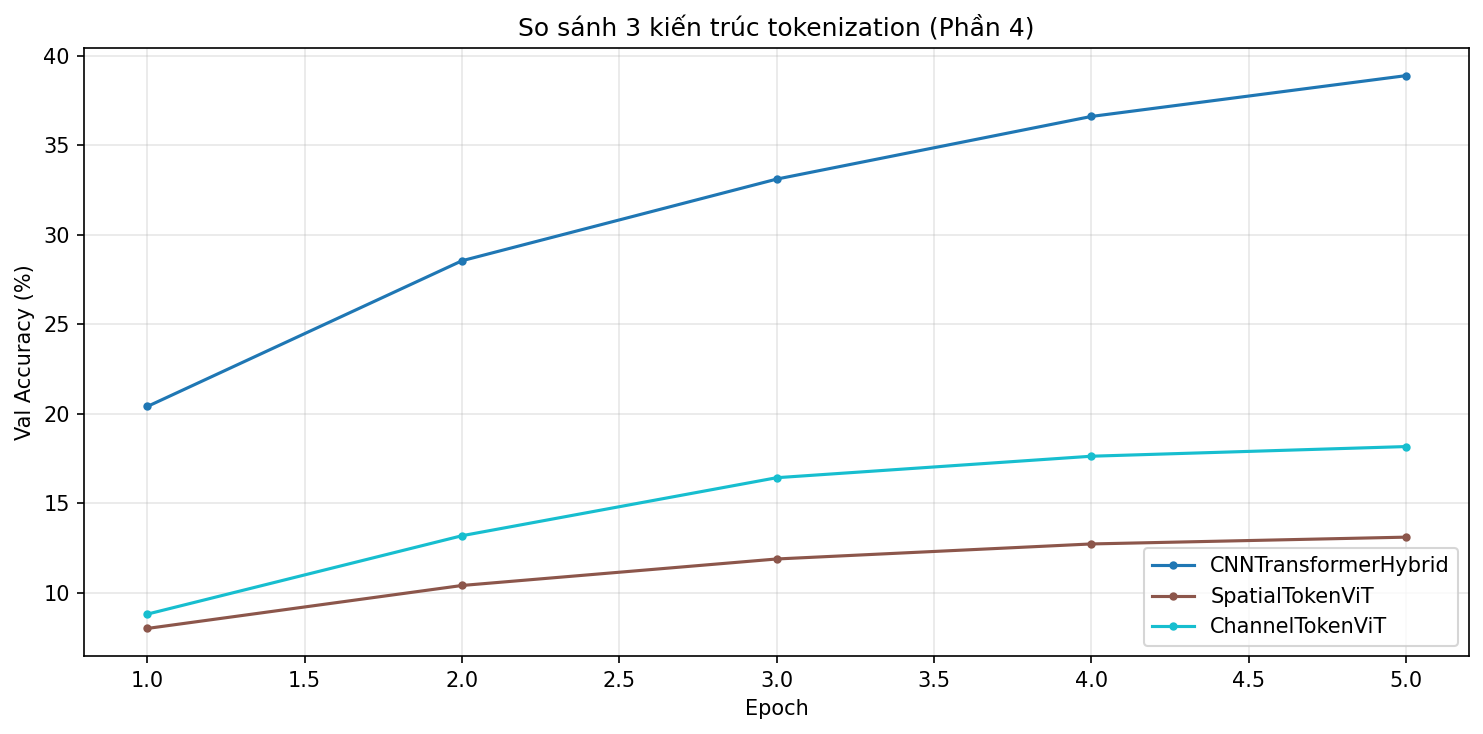
\includegraphics[width=\textwidth]{part4_comparison_curves.png}
    \caption{Training curves}
  \end{subfigure}
  \hfill
  \begin{subfigure}[b]{0.42\textwidth}
    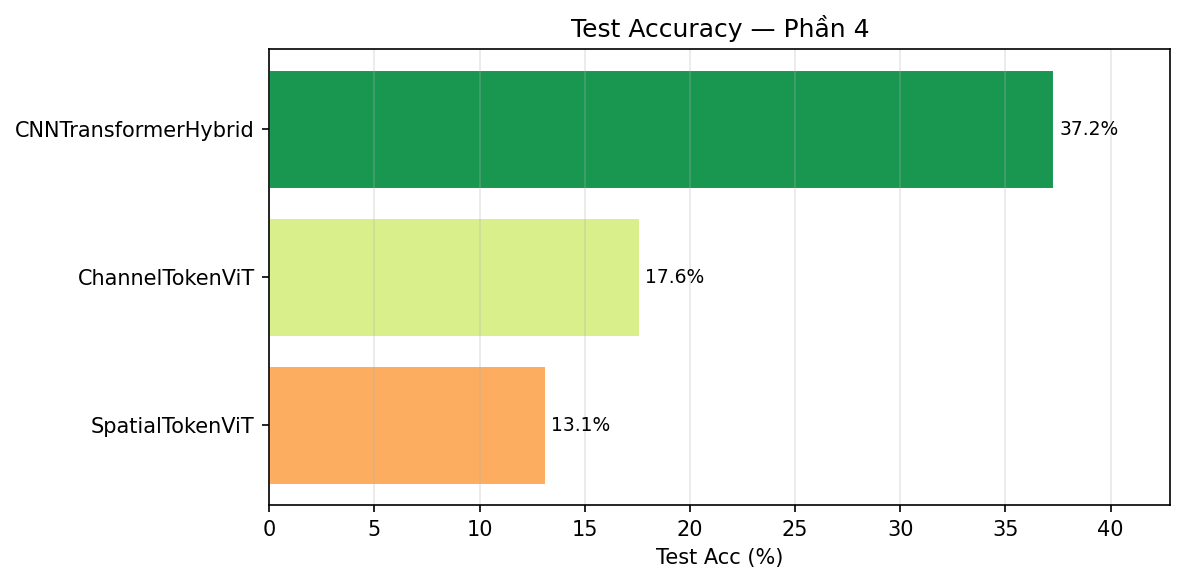
\includegraphics[width=\textwidth]{part4_bar.png}
    \caption{Test Accuracy}
  \end{subfigure}
  \caption{So sánh 3 kiến trúc Phần 4}
\end{figure}

\begin{table}[H]
\centering
\caption{Kết quả Phần 4}
\rowcolors{2}{rowgray}{white}
\begin{tabular}{lcccccc}
\toprule
\textbf{Mô hình} & \textbf{Tokenize} & \textbf{Seq} & \textbf{Test Acc} & \textbf{Val Acc} & \textbf{F1} & \textbf{Params} \\
\midrule
\textbf{CNN+Transformer} & CNN features & 64   & \textbf{37.25\%} & \textbf{38.90\%} & \textbf{35.87\%} & 446.1K \\
ChannelToken ViT         & C channels   & 64   & 17.56\% & 18.18\% & 15.29\% & 549.5K \\
SpatialToken ViT         & H$\times$W pixels & 1,024 & 13.10\% & 13.12\% & 9.86\%  & 172.4K \\
\bottomrule
\end{tabular}
\end{table}

\textbf{Nhận xét:} CNN+Transformer (37.25\%) --- tốt nhất toàn bài. SpatialToken ViT thất bại vì 3 RGB/token quá thô. \textbf{Kết luận: Token quality $>$ Token quantity} --- SpatialToken có $16\times$ nhiều tokens hơn nhưng kết quả tệ hơn $2.8\times$.

% ── 3.5 ──────────────────────────────────────────────────
\subsection{Phần 5 --- LSTM/GRU}

\subsubsection{Biểu diễn ảnh thành chuỗi}

\begin{table}[H]
\centering
\caption{Các cách biểu diễn ảnh thành sequence}
\begin{tabular}{lccl}
\toprule
\textbf{Seq Mode} & \textbf{T} & \textbf{D} & \textbf{Cách biểu diễn} \\
\midrule
Row-wise  & 32 & 96 ($=32\times3$)   & Mỗi hàng pixels \\
Col-wise  & 32 & 96 ($=32\times3$)   & Mỗi cột pixels \\
Patch4    & 64 ($=8\times8$) & 48 ($=4\times4\times3$) & 64 patches $4\times4$ \\
Patch8    & 16 ($=4\times4$) & 192 ($=8\times8\times3$) & 16 patches $8\times8$ \\
\bottomrule
\end{tabular}
\end{table}

\subsubsection{Kiến trúc}

\begin{lstlisting}[style=plainstyle]
Dau vao: [B, T, D]
    |
    v BiLSTM / BiGRU (hidden=256, num_layers=2, bidirectional=True,
                       dropout=0.3)
    v concat(h_n[-2], h_n[-1]) -> [B, 512]
    v Dropout(0.3) -> Linear(512->100) -> [B, 100]
\end{lstlisting}

\begin{table}[H]
\centering
\caption{So sánh LSTM vs GRU}
\begin{tabular}{lll}
\toprule
\textbf{Đặc điểm} & \textbf{LSTM} & \textbf{GRU} \\
\midrule
Số gates        & 4: forget, input, output, cell & 2: reset, update \\
Cell state      & Có ($c_t$)  & Không \\
Params/layer    & $4(D+H)H+4H$ & $3(D+H)H+3H$ \\
Phù hợp         & $T>1000$ steps & $T\leq100$ steps \\
\bottomrule
\end{tabular}
\end{table}

\subsubsection{So sánh}

\begin{figure}[H]
  \centering
  \begin{subfigure}[b]{0.55\textwidth}
    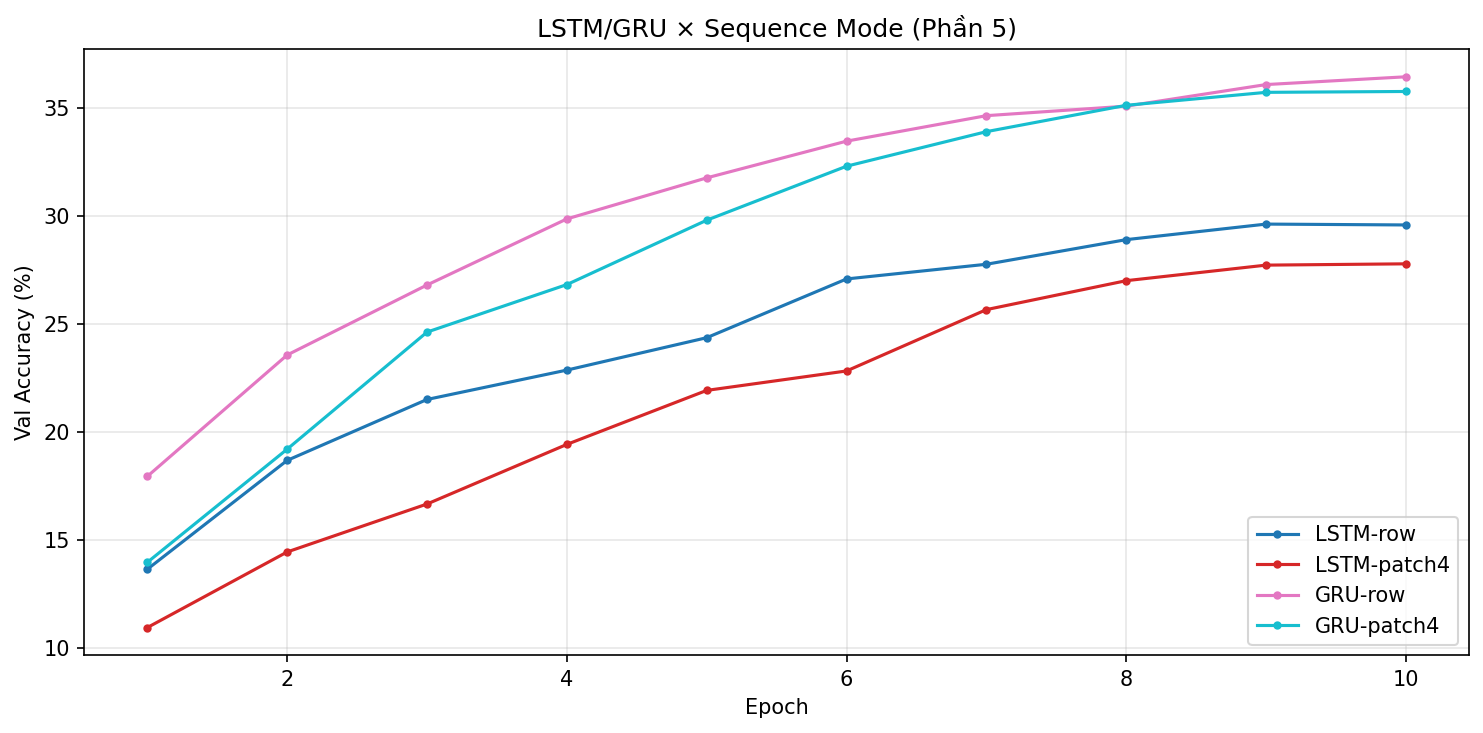
\includegraphics[width=\textwidth]{part5_comparison_curves.png}
    \caption{Training curves}
  \end{subfigure}
  \hfill
  \begin{subfigure}[b]{0.42\textwidth}
    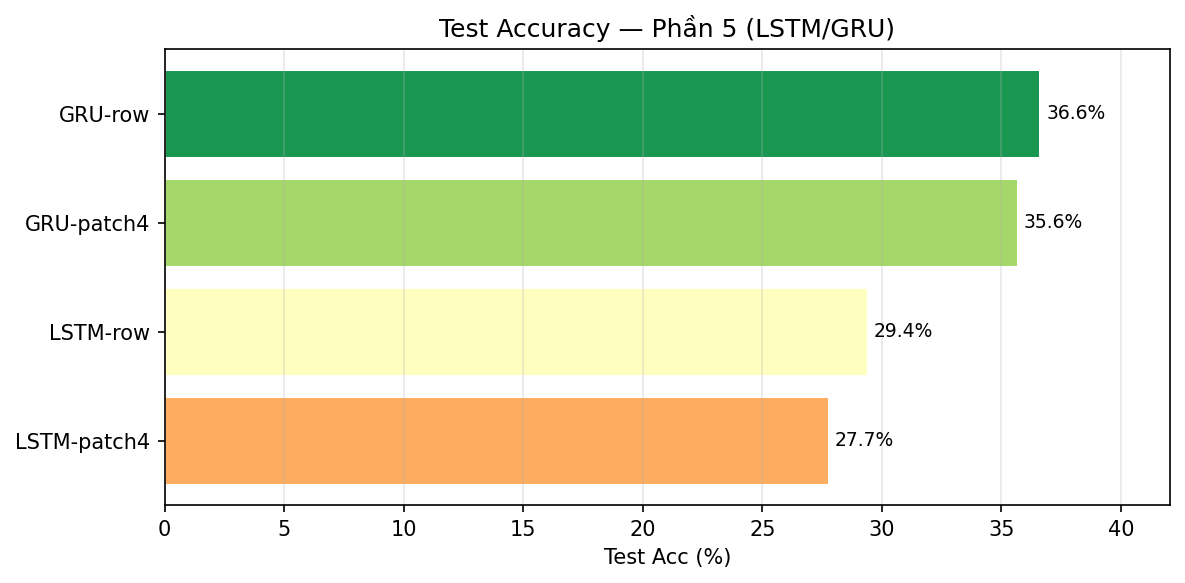
\includegraphics[width=\textwidth]{part5_bar.png}
    \caption{Test Accuracy}
  \end{subfigure}
  \caption{So sánh LSTM và GRU với các cách biểu diễn chuỗi}
\end{figure}

\begin{table}[H]
\centering
\caption{Kết quả Phần 5}
\rowcolors{2}{rowgray}{white}
\begin{tabular}{lcccccc}
\toprule
\textbf{Mô hình} & \textbf{Mode} & \textbf{T} & \textbf{Test Acc} & \textbf{Val Acc} & \textbf{F1} & \textbf{Params} \\
\midrule
\textbf{GRU}  & \textbf{Row} & 32 & \textbf{36.57\%} & \textbf{36.44\%} & \textbf{35.68\%} & 1.8M \\
GRU           & Patch4       & 64 & 35.64\% & 35.76\% & 34.99\% & 1.7M \\
LSTM          & Row          & 32 & 29.36\% & 29.62\% & 28.34\% & 2.4M \\
LSTM          & Patch4       & 64 & 27.73\% & 27.78\% & 26.41\% & 2.3M \\
\bottomrule
\end{tabular}
\end{table}

\textbf{Nhận xét:} GRU vượt LSTM +7.2\% (row) vì chuỗi ngắn $T=32$ không cần cell state riêng biệt của LSTM --- GRU ít params hơn $\rightarrow$ ít overfitting hơn. GRU-row (36.57\%) cạnh tranh ngang SimpleCNN (35.88\%) nhưng cần $5\times$ nhiều tham số hơn.

% ============================================================
\section{Thảo luận}
% ============================================================

\subsection{Bảng xếp hạng toàn bộ 12 mô hình}

\begin{table}[H]
\centering
\caption{Xếp hạng toàn bộ 12 mô hình trên CIFAR-100 test set}
\rowcolors{2}{rowgray}{white}
\small
\begin{tabular}{clllcccc}
\toprule
\textbf{\#} & \textbf{Mô hình} & \textbf{Phần} & \textbf{Kiến trúc} & \textbf{Test Acc} & \textbf{F1} & \textbf{Params} & \textbf{Acc/Param} \\
\midrule
1  & \textbf{CNN+Transformer} & 4 & Hybrid      & \textbf{37.25\%} & 35.87\% & 446.1K  & 83.5\%/M \\
2  & GRU-row                  & 5 & RNN         & 36.57\%          & 35.68\% & 1.8M    & 20.3\%/M \\
3  & \textbf{SimpleCNN}       & 1 & CNN         & 35.88\%          & 34.48\% & \textbf{346.6K} & \textbf{103.5\%/M} \\
4  & GRU-patch4               & 5 & RNN         & 35.64\%          & 34.99\% & 1.7M    & 21.0\%/M \\
5  & CustomViT (tự xây)       & 3 & Transformer & 34.56\%          & 33.11\% & 819.4K  & 42.2\%/M \\
6  & SimpleViT (PyTorch)      & 3 & Transformer & 31.92\%          & 30.39\% & 821.0K  & 38.9\%/M \\
7  & LSTM-row                 & 5 & RNN         & 29.36\%          & 28.34\% & 2.4M    & 12.2\%/M \\
8  & LSTM-patch4              & 5 & RNN         & 27.73\%          & 26.41\% & 2.3M    & 12.1\%/M \\
9  & SimpleViT (Phần 1)       & 1 & Transformer & 24.47\%          & 22.35\% & 821.0K  & 29.8\%/M \\
10 & MLP                      & 1 & FC          & 20.63\%          & 18.31\% & 1.7M    & 12.1\%/M \\
11 & ChannelToken ViT         & 4 & Transformer & 17.56\%          & 15.29\% & 549.5K  & 32.0\%/M \\
12 & SpatialToken ViT         & 4 & Transformer & 13.10\%          &  9.86\% & 172.4K  & 76.0\%/M \\
13 & SoftmaxRegression        & 1 & Linear      &  7.94\%          &  6.09\% & 307.3K  & 25.8\%/M \\
\bottomrule
\end{tabular}
\end{table}

\subsection{CNN vs ViT}

\begin{table}[H]
\centering
\caption{So sánh CNN và ViT}
\begin{tabular}{lll}
\toprule
\textbf{Khía cạnh} & \textbf{CNN} & \textbf{ViT} \\
\midrule
Inductive bias     & Locality + weight sharing  & Không có \\
Data requirement   & Thấp                       & Cao (cần pretrain) \\
Accuracy (bài này) & 35.88\%                    & 24.47\%--31.92\% \\
Efficiency         & 103.5\%/M                  & 29.8\%--42.2\%/M \\
Receptive field    & Tăng dần theo layers       & Global từ layer 1 \\
Phù hợp            & Small datasets             & Large-scale pretraining \\
\bottomrule
\end{tabular}
\end{table}

\textbf{Kết luận:} Với CIFAR-100 (45K mẫu, from scratch), CNN chiếm ưu thế nhờ inductive bias phù hợp. ViT thực sự vượt CNN khi pretrained trên ImageNet-21K (14M ảnh) --- không phải kiến trúc kém, mà thiếu data.

\subsection{Transformer vs RNN}

\begin{table}[H]
\centering
\caption{So sánh Transformer và RNN}
\begin{tabular}{lll}
\toprule
\textbf{Khía cạnh} & \textbf{Transformer} & \textbf{RNN (LSTM/GRU)} \\
\midrule
Cơ chế             & Self-Attention (toàn cục, song song) & Recurrence (tuần tự) \\
Long-range dependency & $O(1)$ --- mọi cặp token trực tiếp & $O(T)$ --- lan truyền qua steps \\
Parallelism        & Cao                   & Thấp \\
Memory             & $O(T^2)$ attention    & $O(T)$ hidden states \\
Kết quả (bài này)  & ViT: 24--34\%         & GRU: 35--36\%, LSTM: 27--29\% \\
\bottomrule
\end{tabular}
\end{table}

\subsection{Trade-off: Accuracy, tốc độ và data requirement}

\begin{table}[H]
\centering
\caption{Trade-off tổng hợp}
\begin{tabular}{lcccl}
\toprule
\textbf{Kiến trúc} & \textbf{Accuracy} & \textbf{Time/ep} & \textbf{Data req.} & \textbf{Phù hợp} \\
\midrule
CNN                 & $\sim$36\% & $\sim$15s & Thấp     & Small dataset, production \\
CNN+Transformer     & $\sim$37\% & $\sim$20s & Trung bình & Cần global context \\
GRU                 & $\sim$36\% & $\sim$25s & Trung bình & Sequential patterns \\
ViT (from scratch)  & $\sim$31\% & $\sim$45s & Cao       & Pretrain available \\
LSTM                & $\sim$28\% & $\sim$30s & Trung bình & Long sequences \\
Softmax/MLP         & 8--21\%   & $\sim$5s  & Thấp      & Baseline only \\
\bottomrule
\end{tabular}
\end{table}

% ============================================================
\section{Kết luận}
% ============================================================

\subsection{Mô hình tốt nhất}

\textbf{CNN+Transformer Hybrid} đạt test accuracy cao nhất (37.25\%), kết hợp spatial inductive bias từ CNN và global attention từ Transformer.

\textbf{SimpleCNN} là lựa chọn tốt nhất xét về \textbf{hiệu quả tham số} (103.5\%/M): chỉ 346.6K params, huấn luyện nhanh, không cần tuning phức tạp.

\subsection{Insight chính}

\begin{enumerate}
  \item \textbf{Inductive bias phù hợp quan trọng hơn model size:} SimpleCNN (346.6K) vượt MLP (1.7M) và LSTM (2.4M). Kiến trúc phù hợp với cấu trúc dữ liệu hiệu quả hơn chỉ tăng số tham số.

  \item \textbf{ViT cần data lớn để hội tụ tốt:} Với 45K mẫu from scratch, ViT (24--34\%) thua CNN (36--37\%). ViT thực sự vượt CNN khi pretrained trên tập lớn.

  \item \textbf{Hybrid kết hợp được hai thế mạnh:} CNN+Transformer đạt 37.25\% bằng cách dùng CNN tạo tokens chất lượng cao rồi Transformer học quan hệ toàn cục.

  \item \textbf{Token quality $>$ token quantity:} SpatialToken ViT (1,024 raw pixel tokens $\rightarrow$ 13.10\%) thua CNN features (64 high-quality tokens $\rightarrow$ 37.25\%). $16\times$ nhiều tokens nhưng kết quả tệ hơn $2.8\times$.

  \item \textbf{GRU $\geq$ LSTM cho chuỗi ngắn:} Với $T=32$--64, GRU ít params hơn $\rightarrow$ ít overfitting $\rightarrow$ kết quả tốt hơn LSTM.
\end{enumerate}

\subsection{Hướng cải thiện tiếp theo}

\begin{itemize}
  \item \textbf{Data augmentation mạnh hơn:} CutMix, MixUp, RandAugment $\rightarrow$ dự kiến +5--10\% accuracy.
  \item \textbf{LR warmup cho ViT:} Linear warmup 10 epochs trước CosineAnnealing.
  \item \textbf{Deeper CNN backbone:} Residual connections (ResNet-style) $\rightarrow$ target $>$50\% test accuracy.
  \item \textbf{Pre-trained features:} Dùng CLIP/DINO features thay vì train from scratch.
  \item \textbf{Label smoothing} ($\varepsilon=0.1$): Regularize CrossEntropyLoss cho 100 lớp.
\end{itemize}

% ============================================================
\section{Tài liệu tham khảo}
% ============================================================

\begin{enumerate}
  \item Dosovitskiy, A. et al. (2021). \textit{An Image is Worth 16$\times$16 Words: Transformers for Image Recognition at Scale}. ICLR 2021.
  \item Vaswani, A. et al. (2017). \textit{Attention Is All You Need}. NeurIPS 2017.
  \item He, K. et al. (2016). \textit{Deep Residual Learning for Image Recognition}. CVPR 2016.
  \item Simonyan, K. \& Zisserman, A. (2015). \textit{Very Deep Convolutional Networks for Large-Scale Image Recognition (VGGNet)}. ICLR 2015.
  \item Cho, K. et al. (2014). \textit{Learning Phrase Representations using RNN Encoder-Decoder for Statistical Machine Translation}. EMNLP 2014.
  \item Chung, J. et al. (2014). \textit{Empirical Evaluation of Gated Recurrent Neural Networks on Sequence Modeling}. arXiv 2014.
  \item Krizhevsky, A. (2009). \textit{Learning Multiple Layers of Features from Tiny Images}. Technical Report, University of Toronto.
  \item Touvron, H. et al. (2021). \textit{Training data-efficient image transformers \& distillation through attention (DeiT)}. ICML 2021.
  \item Ba, J. et al. (2016). \textit{Layer Normalization}. arXiv 2016.
\end{enumerate}

\vspace{2em}
\hrule
\vspace{0.5em}
\small\textit{Báo cáo hoàn thành ngày 31/03/2026 \textbar{} CO5085 – Học sâu và ứng dụng trong thị giác máy tính \textbar{} HCMUT}

\end{document}
